%%%%%%%%%%%%%%%%%%%%%%%%%%%%%%%%%%%%%%%%%
% University/School Laboratory Report
% LaTeX Template
% Version 3.1 (25/3/14)
%
% This template has been downloaded from:
% http://www.LaTeXTemplates.com
%
% Original author:
% Linux and Unix Users Group at Virginia Tech Wiki 
% (https://vtluug.org/wiki/Example_LaTeX_chem_lab_report)
%
% License:
% CC BY-NC-SA 3.0 (http://creativecommons.org/licenses/by-nc-sa/3.0/)
%
%%%%%%%%%%%%%%%%%%%%%%%%%%%%%%%%%%%%%%%%%

%----------------------------------------------------------------------------------------
%	PACKAGES AND DOCUMENT CONFIGURATIONS
%----------------------------------------------------------------------------------------

\documentclass{article}

%\usepackage[version=3]{mhchem} % Package for chemical equation typesetting
\usepackage{graphicx} % Required for the inclusion of images
\usepackage{natbib} % Required to change bibliography style to APA
\usepackage{amsmath} % Required for some math elements 
\usepackage[utf8]{inputenc} % Required for special characters processing
\usepackage{url}
%
\usepackage{fullpage} % changes the margin
\usepackage{siunitx} % Provides the \SI{}{} and \si{} command for typesetting SI units
\newcommand{\gc}{\degreeCelsius}
\usepackage{pdflscape} % Change text sections orientation
%
\setlength\parindent{0pt} % Removes all indentation from paragraphs

\renewcommand{\labelenumi}{\alph{enumi}.} % Make numbering in the enumerate environment by letter rather than number (e.g. section 6)

\usepackage{times} % Uncomment to use the Times New Roman font

%----------------------------------------------------------------------------------------
%	DOCUMENT INFORMATION
%----------------------------------------------------------------------------------------

\title{\textbf{Surface Pressure Charts and  Meteorology Codes} \\ Meteorology
  \& Climatology} % Title

\author{Environmental Science Degree} % Author name

\date{\today} % Date for the report

\begin{document}

\maketitle % Insert the title, author and date

\begin{center}
\begin{tabular}{l r}
Date Performed: & \underline{\hspace{3cm}}  \\ % Date the experiment was performed
Partners: & \underline{\hspace{6cm}} \\ % Partner names
& \underline{\hspace{6cm}} \\
& \underline{\hspace{6cm}} \\
Instructor: & Prof.~F.~Pérez-Bernal % Instructor/supervisor
\end{tabular}
\end{center}

% If you wish to include an abstract, uncomment the lines below
\begin{abstract}
This lab session aim is that students understand isobars and their relationship with wind speed,
identify various pressure systems and fronts on a weather chart, and 
interpret and produce plotted weather symbols. For the latter case  meteorology report codes, in
particular the SYNOP code, is presented. Students should
learn to encode a general weather situation to this code as well as to
interpret the code both graphically and as a short weather report.
\end{abstract}

%----------------------------------------------------------------------------------------
%	SECTION 1
%----------------------------------------------------------------------------------------
\section{Introduction}
% is a format for reporting weather information. A METAR weather
% report is predominantly used by pilots in fulfillment of a part of a
% pre-flight weather briefing, and by meteorologists, who use
% aggregated METAR information to assist in weather forecasting.
Surface pressure charts show the surface pressure pattern using
\textit{isobars} (a particular kind of \textit{isopleths}, solid lines joining points of equal sea level pressure) and
indicate areas of high ($H$) and low pressure ($L$) along with their
central pressure value. High pressure is usually associated with
settled weather while low pressure is normally associated with
unsettled weather. 

In these charts fronts and other information of meteorological
interest can be also displayed. In particular, in the so called
\textit{synoptic charts} an extensive information about the state of
the atmosphere, usually reported with a graphical transcription of the SYNOP
code, is graphically encoded and represented.

SYNOP stands for \textit{surface SYNOPtic observation} and it is a
numerical code (called FM-12 by the World Meteorological Office
WMO\cite{WMOFM-12,FM-12}) that has been used for decades as the main way of
reporting and transmitting weather information. The observations could
be made by manned and automated weather stations.

The international SYNOP format has been used for real time
transmission of synoptic weather observations for about 50 years and
SYNOP reports are typically sent every six hours by Deutscher
Wetterdienst on shortwave and low frequency using RTTY. The
introduction of Internet made this redundant.

A report consists  of groups of five numbers (and slashes
where data are not  available) describing general weather information,
such  as  the temperature,  atmospheric  pressure, precipitation,  and
visibility at a weather station.

In most countries, SYNOP observations are made and transmitted each 3
hours at 0000, 0300, 0600, 0900, 1200, 1500, 1800, and 2100 Universal
Time (UTC). There are two basic forms of land station surface synoptic
reports, one of which is the complete form and the other is the
shortened form. The complete form is referred to as the primary (or
main) synoptic, the 6-hourly report, or SYNOP. The primary synoptic is
reported at the standard hours of observation which are: 0000, 0600,
1200, and 1800 UTC. The shortened form is referred to as the
intermediate synoptic or the 3-hourly report.

The SYNOP code is very similar to another code called the METAR. METAR
is an abbreviation of \textit{MÉTéorologique Aviation Régulière} and
is a report designed for aviation that could be issued from an
Automatic Weather Station (AWS) or a manned station. The METAR code is
also managed by the WMO. METARs usually carry less information about
the weather than SYNOPs and are issued more frequently. In particular,
if conditions change significantly since the last METAR, a SPECI, or
special weather report is produced. SPECIs are sent to report heavy
rain, sudden increase or direction change of wind, strong gusts, or
sudden temperature or visibility variations.

\section{Objectives}
The objectives of this lab session are the following:
\begin{enumerate}
\item Understand surface pressure maps and their relationship
  with wind speed.
\item Identify pressure systems and fronts on a synoptic weather
  chart.
\item Get acquainted with the SYNOP code to interpret and produce plotted
  weather symbols.
\end{enumerate}

\section{Isobars, pressure and winds}
Isobar lines join points of equal pressure, in a similar way to height
contours, on weather charts. Charts showing isobars help to identify
anticyclones (high atmospheric pressure areas) and depressions or
cyclones (low pressure areas). Pressure is measured in
millibars\footnote{Remember: \SI{1}{mb} = \SI{1}{hPa}} and isobars are
normally drawn at intervals of $\Delta p = \SI{4}{mb}$. Pressure
values are corrected to Mean Sea Level Pressure (MSLP) before being
plotted on a map, this ensures that altitude does not affect the
mapping.

Drawing isobars in a map it is important to take into account the
following considerations.

\begin{itemize}
\item Each map point can only be associated with one isobar, thus
  isobar lines never cross. 
\item Isobar lines are continuous, forming loops or terminating in the
  map edges, but never branch or terminate in a certain point.
\item A particular sense can be given to an isobar considering that
  the pressure should grow to the right of the given sense.
\end{itemize} 

Isobars are also helpful because their distribution helps us to
understand the direction and strength of wind in a particular
location. Where isobars are \textit{close together}, for example near
a low pressure area, they indicate \textit{strong} winds. Where the
isobars are more \textit{widely spaced}, e.g.\ near an anticyclone,
they indicate \textit{light} winds.

Wind blows almost parallel to the isobars. Around a high pressure area
(an anticyclone) winds  blow clockwise and slightly across the isobars, away from
the center of the anticyclone. In low pressure zones, wind blows
anticlockwise slightly across the isobars towards the cent-re of the low pressure.

\textit{Buys Ballot’s law} states that if you stand with your back to
the wind in the northern Hemisphere, low pressure will be on your
left. With the help of this law that you can work out the wind direction at different
locations on a weather chart.

There are several features of weather chart that can be easily
identified.

An \textit{anticyclone}, also known as a ‘high’ can be identified on a
weather chart as an (often large) area of widely spaced isobars, where
pressure is higher than in the surrounding area and the highest pressure
occurs at the center which is known as the ‘high pressure
center’. Anticyclones can bring warm and sunny weather in summer, but
cold and foggy weather in winter. In association with anticyclones,
\textit{ridges} are elongated extensions of areas of high
pressure. They bring similar weather to that associated with
anticyclones.

A \textit{cyclone}, also known as a depression or a ‘low’ can be recognized on a weather
chart by an area of closely spaced isobars, often in a roughly
circular shape, where pressure is lower than surrounding areas. They
are often accompanied by fronts. The lowest pressure occurs at the
'low pressure center', in the middle of a depression. Cyclones are
often associated with strong winds and heavy rain and are nearly
always accompanied by fronts. Associated with cyclones,
\textit{troughs} are elongated extensions of areas of low
pressure and bring similar weather to that associated with
depressions. 


\textit{Cold fronts} can be identified on weather charts as bold lines
with triangles. These are blue when displayed on color charts. The
points of the triangle indicate the direction in which the front is
moving. A cold front indicates a change in air mass, where warmer air
is being replaced by colder air. They often bring short spells of
heavy rainfall in the form of showers and squally winds, and are
accompanied by a decrease in temperature, a veer in wind direction and
a change to brighter showery conditions. 

\textit{Warm fronts} can be identified on weather charts as bold lines
with semi-circles or humps. These are colored red when displayed on
color charts. The direction of the humps indicates the direction in
which the front is moving. A warm front indicates a change from a
colder to a warmer air mass. They often bring spells of prolonged and
sometimes heavy rainfall, with strong winds. 

The warm sector of a depression is located behind the warm front and
ahead of the cold front. It often brings mild temperatures but the
weather can be overcast with drizzle.

\textit{Occluded fronts} can be identified on weather charts as bold
lines with sets of triangles and semi-circles. These are colored
purple on colored weather charts. The direction in which the symbols
face indicates the direction in which the front is
traveling. Occlusions are formed when the cold front overtakes the
warm front, therefore they have similar characteristics to a cold
front, but less intense.

Other features of interest are \textit{troughs} and \textit{cols}.
\textit{Troughs} are lines of low
pressure and high vorticity, with clouds, and possible precipitation, wind
shift and confluence. They often do not possess the strong horizontal
gradients of temperature and moisture that characterize fronts. \textit{Cols} can be identified as an area of slack pressure between two anticyclones and two depressions.


\section{Synop Code Description}


The SYNOP code data are divided in  four main groups:

\begin{description}
\item{000 Group} Data Identifier
\item{111 Group} Land Observations
\item{222 Group} Sea Surface Observations
\item{333 Group} Climatological Data
\end{description}




Most reports do not make use all of the groups. For example, only at a coastal station would the section 222 (wave
information) be included, and even that station might not include all of the groups in the 222
section. Also, individual groups may be left out of an observation for a number of reasons.
Different regions may have requirements which will include groups or exclude groups,
principally in section 333.

We will deal with land synoptic reports is the first group, which are often stated as $AAXX$ and are compliant with the WMO Code FM 12 XI SYNOP.  The general syntax of the SYNOP code for such reports is as follows
\begin{align*}
&YYGGi_w\; IIiii \text{ or } IIIII\;  99LLL\; QLLLL\\
&i_Ri_XhVV\; Nddff\; 00fff\; 1sTTT\; 2sTTT\; 3PPPP\; 4PPPP\; 5appp\; 6RRRt\; 7wwW_1W_2\; 8NC_LC_MC_H\; 9GGgg\\
&222Dv\; 0sTTT\; 1PPHH\; 2PPHH\; 3dddd\; 4PPHH\; 5PPHH\; 6IEER\; 70HHH\; 8aTTT\\
&333\; 0....\; 1sTTT\; 2sTTT\; 3Ejjj\; 4Esss\; 5jjjj\; jjjjj\; 6RRRt\; 7RRRR\; 8Nchh\; 9SSss
\end{align*}


\subsection{000 Group: Identification and Location}

\begin{description}
\item[$\pmb{YYGGi_w}$]
  \begin{tabular}{cl}
    $YY$ & The day of the month\\
    $GG$ & The hour of the observation (UTC)\\
    $i_w$ & Wind type indicator\\
    0  & m/s (estimated)\\
    1  & m/s (from anemometer)\\
    3  & knots (estimated)\\
    4  & knots (from anemometer)
  \end{tabular}
\item[$\pmb{IIiii}$] The WMO number of the station\footnote{In order to check station codes visit the url \url{http://weather.rap.ucar.edu/surface/stations.txt} or make a query at NOAA website \url{http://www.nws.noaa.gov/tg/siteloc.php}.}\nocite{stindex}.
\item[$\pmb{IIIII}$] Ship or Buoy Observations.The ship or buoy identifier. (Not reported in land observations)
\item[$\pmb{99LLL~QLLLL}$] Observation location. (Not reported in fixed land station)
  \begin{tabular}{cl}
    $LLL$ & Latitude of observation to $0.1$ degrees\\
    $Q$ & Quadrant of observation\\
    1 & North east \\
    3 & South east\\
    5 & South west\\
    7 & North west\\
    $LLLL$ & Longitude of  observation to $0.1$ degrees
  \end{tabular}
\end{description}

\subsection{111 Group: Land Observations}

\begin{description}
\item[$\pmb{i_Ri_XhVV}$]
  \begin{description}
  \item[$i_R$] -- Precipitation indicator
    \begin{tabular}{cl}
      0 & Precipitation in groups 1 and 3\\
      1 & Precipitation reported in group 1 only\\
      2 & Precipitation reported in group 3 only\\
      3 & Precipitation omitted, no precipitation\\
      4 & Precipitation omitted, no observation
    \end{tabular}
  \item[$i_X$] -- Station type and present/past weather indicator
    \begin{tabular}{cll}
      Value & Station & Weather group\\
      1 & manned  &included\\
      2 & manned  &omitted, no significant weather\\
      3 & manned  &omitted, no weather observation\\
      4 & automated  & included (see automated codes 4677 and 4561)\\
      5 & automated  & omitted, no significant weather\\
      6 & automated  & omitted, no weather observation\\
      7 & automated  & included (see automated codes 4680 and 4531)\\
    \end{tabular}
  \item[$h$] -- Cloud base of lowest cloud seen (meters above ground)
    \begin{tabular}{cl}
      0 & 0 to 50 m \\
      1 & 50 to 100 m \\
      2 & 100 to 200 m\\
      3 & 200 to 300 m\\
      4 & 300 to 600 m\\
      5 & 600 to 1000 m\\
      6 & 1000 to 1500 m\\
      7 & 1500 to 2000 m\\
      8 & 2000 to 2500 m\\
      9 & above 2500 m\\
      / & unknown\\
    \end{tabular}
  \item[$VV$] -- Visibility
    \begin{tabular}{lllll}
      00 $<$ 0.1 km & 01 -- 0.1 km & 02 -- 0.2 km & ... & 50 -- 5.0 km\\
      56 -- 6 km          & 57 -- 7 km   & 58 -- 8 km   & ... & 80 -- 30 km \\
      81 -- 35 km         & 82 -- 40 km  & 83 -- 45 km  & 84 -- 50 km & 85 -- 55 km\\
      86 -- 60 km         & 87 -- 65 km  & 88 -- 70 km  & 89 -- $>$ 70 km & \\
      90 -- $<$ 0.05 km     &91 -- 0.05 km & 92 -- 0.2 km & 93 -- 0.5 km & 94 -- 1 km\\
      95 -- 2 km          &96 -- 4 km    & 97 -- 10 km & 98 -- 20 km & 99 -- $>$ 50 km\\
      // -- missing       &              &             &             &               \\
    \end{tabular}
  \end{description}
\end{description}
\begin{description}
\item[$\pmb{Nddff}$]
  \begin{description}
  \item[$ N$] -- Total cloud cover
    \begin{tabular}{llllll}
      0 -- clear & 1 -- 1/8th & 2 -- 2/8ths & 3 -- 3/8ths &  4 -- 4/8ths& 5 -- 5/8ths \\
      6 -- 6/8ths& 7 -- 7/8ths & 8 -- overcast & 9 -- sky obscured & &/ -- no observation
    \end{tabular}
  \end{description}
\item[$dd$] -- wind direction in 10s of degrees 
\item[$ff$] -- wind speed in units determined by wind type indicator (see above)
\end{description}
\begin{description}
\item[$\pmb{00fff}$ (optional)]
  \begin{description}
  \item[$fff$] -- wind speed if value greater than 100
  \end{description}
\end{description}
\begin{description}
\item[$\pmb{1sTTT}$] -- Temperature
  \begin{description}
  \item[$s$] -- sign of temperature (0=positive, 1=negative)
  \item[$TTT$] -- Temperature in \SI{0.1}{\gc}
  \end{description}
\end{description}
\begin{description}
\item[$\pmb{2sTTT}$] -- Dew point
    \begin{description}
    \item[$s$] -- sign of temperature (0=positive, 1=negative, 9 = RH)
    \item[$TTT$] -- Dew point temperature in \SI{0.1}{\gc} (if $s$ is 9, $TTT$ is relative humidity)
  \end{description}
\end{description}
\begin{description}
\item[$\pmb{3PPPP}$] -- Station pressure in \SI{0.1}{hPa} (thousandths digit omitted, last digit can be slash, then pressure in full \si{hPa})
\end{description}
\begin{description}
\item[$\pmb{4PPPP}$] -- Sea level pressure in \SI{0.1}{hPa} (thousandths digit omitted, last digit can be slash, then pressure in full \si{hPa})
\end{description}
\begin{description}
\item[$\pmb{4a_3hhh}$] -- Geopotential of nearest mandatory pressure level (use for high altitude stations where sea level pressure reduction is not accurate)
  
  \begin{description}
  \item[$a_3$] -- -- mandatory pressure level
    \begin{tabular}{lll}
      1 -- 1000 mb & 2 -- 925 m &5 -- 500 mb\\
      7 -- 700 mb  & 8 -- 850 mb& hhh -- geopotential height omitting thousandths digit
    \end{tabular}
  \end{description}
\end{description}

\begin{description}
\item[$\pmb{5appp}$] -- Pressure tendency over 3 hours
  \begin{description}
  \item[$a$] -- characteristics of pressure tendency
    \begin{tabular}{l}
      0 -- Increasing, then decreasing -- resultant pressure same or higher\\
      1 -- Increasing, then steady -- resultant pressure higher\\
      2 -- Increasing steadily -- resultant pressure higher\\
      3 -- Decreasing or steady, then increasing -- resultant pressure higher\\
      4 -- Steady -- resultant pressure same\\
      5 -- Decreasing, then increasing -- resultant pressure lower\\
      6 -- Decreasing, then steady -- resultant pressure lower\\
      7 -- Decreasing steadily -- resultant pressure lower\\
      8 -- Increasing or steady, then decreasing -- resultant pressure lower\\
    \end{tabular}
  \item[$ppp$] -- 3 hour pressure change in 0.1 mb
  \end{description}
\end{description}
\begin{description}
\item[$\pmb{6RRRt}$] -- Liquid precipitation
  \begin{description}
  \item[$RRR$] -- Precipitation amount in mm

    \begin{tabular}{lllll}
      001 -- 1 mm&002 -- 2 mm&...&988 -- 988 mm&989 -- 989 or more mm\\
      990 -- Trace&991 -- 0.1 mm&992 -- 0.2 mm&...&999 -- 0.9 mm
    \end{tabular}
  \item[$t$] -- Duration over which precipitation amount measured

    \begin{tabular}{lll}
      1 -- 6 hours&2 -- 12 hours&3 -- 18 hours\\
      4 -- 24 hours&5 -- 1 hour& 6 -- 2 hours\\
      7 -- 3 hours&8 -- 9 hours&9 -- 15 hours\\
      / -- 24 hours& &
    \end{tabular}
  \end{description}
\end{description}
\begin{description}
\item[$\pmb{7wwW_1W_2}$] -- Present and past weather
  \begin{description}  
  \item[$ww$] The present weather codes can be found in the next page.

  \item[$W_1W_2$] -- Past weather (type 1 and 2)

    \begin{tabular}{l}
      0 -- cloud covering less than half of sky\\
      1 -- cloud covering more than half of sky during part of period and more than half during part of period\\
      2 -- cloud covering more than half of sky\\
      3 -- sandstorm, dust storm or blowing snow\\
      4 -- fog, or thick haze\\
      5 -- drizzle\\
      6 -- rain\\
      7 -- snow or mixed rain and snow\\
      8 -- showers\\
      9 -- thunderstorms
    \end{tabular}
  \end{description}
\end{description}
\begin{description}
  \item[$\pmb{8NC_LC_MC_H}$] -- Cloud type information
    \begin{description}
      \item[$N$] -- Amount of low clouds covering sky, if no low clouds, the amount of the middle clouds
      \item[$C_L$] -- Low cloud type

        \begin{tabular}{ll}
          0 -- no low clouds& 1 -- cumulus humulis or fractus (no vertical development)\\
          \multicolumn{2}{l}{2 -- cumulus mediocris or congestus (moderate vertical development)}\\
          3 -- cumulonimbus calvus (no outlines nor anvil)&4 -- stratocumulus cumulogenitus (formed by spreading of cumulus)\\
          5 -- stratocumulus& 6 -- stratus nebulosus (continuous sheet)\\
          7 -- stratus or cumulus fractus (bad weather)&8 -- cumulus and stratocumulus (multilevel)\\
          9 -- cumulonimbus with anvil&/ -- low clouds unobserved due to darkness or obscuration
        \end{tabular}
      \item[$C_M$] -- Middle cloud type
        
        \begin{tabular}{ll} 
         0 -- no middle clouds&1 -- altostratus translucidous (mostly transparent)\\
          2 -- altostratus opacus or nimbostratus&3 -- altocumulus translucidous (mostly transparent)\\
          4 -- patches of altocumulus (irregular, lenticular)&5 -- bands of altocumulus\\
          \multicolumn{2}{l}{6 -- altocumulus cumulogenitus (formed by spreading of cumulus)}\\
          7 -- altocumulus (multilayers)&8 -- altocumulus castellanus (having cumuliform tufts)\\
          9 -- altocumulus of a chaotic sky&/ -- middle clouds unobserved due to darkness or obscuration \\
        \end{tabular}
      \item[$C_H$] -- High cloud type

        \begin{tabular}{ll}
          0 -- no high clouds&1 -- cirrus fibratus (wispy)\\
          2 -- cirrus spissatus (dense in patches)&3 -- cirrus spissatus cumulogenitus (formed out of anvil)\\
          4 -- cirrus unicus or fibratus (progressively invading sky) &\\
          \multicolumn{2}{l}{5 -- bands of cirrus or cirrostratus invading sky (less than 45$^\circ$ above horizon)}\\
          \multicolumn{2}{l}{6 -- bands of cirrus or cirrostratus invading sky (more than 45$^\circ$ above horizon)}\\
          7 -- cirrostratus covering whole sky&8 -- cirrostratus not covering sky but not invading\\
          9 -- cirrocumulus &/ -- high clouds unobserved due to darkness or obscuration \\
      \end{tabular}
\end{description}
\end{description}

\begin{description}
\item[$\pmb{9GGgg}$] -- Time of observation in hours and minutes (Optional)
\end{description}
%\newpage
\begin{landscape}

      \pagenumbering{gobble}
      \hspace{-1cm}
      {\small
        \begin{tabular}{llll}
          \multicolumn{4}{l}{$ww$ -- \textbf{Present weather}}\\
        00 -- clear skies&01 -- clouds dissolving&02 -- state of sky unchanged&03 -- clouds developing\\
        \multicolumn{4}{l}{Haze, smoke, dust or sand}\\
        04 -- visibility reduced by smoke&05 -- haze&\multicolumn{2}{l}{06 -- widespread dust in suspension not raised by wind}\\
        07 -- dust or sand raised by wind&08 -- well developed dust or sand whirls&\multicolumn{2}{l}{09 -- dust or sand storm within sight but not at station}\\
        \multicolumn{4}{l}{Non-precipitation events}\\
        10 -- mist&11 -- patches of shallow fog&12 -- continuous shallow fog&13 -- lightning visible, no thunder heard\\
        \multicolumn{2}{l}{14 -- precipitation within sight but not hitting ground}&      \multicolumn{2}{l}{15 -- distant precipitation but not falling at station}\\
        \multicolumn{2}{l}{16 -- nearby precipitation but not falling at station}&\multicolumn{2}{l}{17 -- thunderstorm but no precipitation falling at station}\\
        \multicolumn{2}{l}{18 -- squalls within sight but no precipitation falling at station}&\multicolumn{2}{l}{19 -- funnel clouds within sight}\\
        \multicolumn{4}{l}{Precipitation within past hour but not at observation time}\\
        20 -- drizzle&21 -- rain&22 -- snow&23 -- rain and snow\\
        24 -- freezing rain&25 -- rain showers&26 -- snow showers&27 -- hail showers\\
        28 -- fog& 29 -- thunderstorms& & \\
        \multicolumn{4}{l}{Dust storm, sandstorm, drifting or blowing snow}\\
        \multicolumn{2}{l}{30 -- slight to moderate dust storm, decreasing in intensity}&\multicolumn{2}{l}{31 -- slight to moderate dust storm, no change}\\
        \multicolumn{2}{l}{32 -- slight to moderate dust storm, increasing in intensity}&\multicolumn{2}{l}{33 -- severe dust storm, decreasing in intensity}\\
        \multicolumn{2}{l}{34 -- severe dust storm, no change}&\multicolumn{2}{l}{35 -- severe dust storm, increasing in intensity}\\
        \multicolumn{2}{l}{36 -- slight to moderate drifting snow, below eye level}&\multicolumn{2}{l}{37 -- heavy drifting snow, below eye level}\\
        \multicolumn{2}{l}{38 -- slight to moderate drifting snow, above eye level}&\multicolumn{2}{l}{39 -- heavy drifting snow, above eye level}\\
        \multicolumn{4}{l}{Fog or ice fog}\\
        40 -- Fog at a distance&41 -- patches of fog&42 -- fog, sky visible, thinning&43 -- fog, sky not visible, thinning\\
        44 -- fog, sky visible, no change&45 -- fog, sky not visible, no change&46 -- fog, sky visible, becoming thicker&47 -- fog, sky not visible, becoming thicker\\
        48 -- fog, depositing rime, sky visible&49 -- fog, depositing rime, sky not visible& & \\
        \multicolumn{4}{l}{Drizzle}\\
        50 -- intermittent light drizzle&51 -- continuous light drizzle&52 -- intermittent moderate drizzle&53 -- continuous moderate drizzle\\
        54 -- intermittent heavy drizzle&55 -- continuous heavy drizzle&56 -- light freezing drizzle&57 -- moderate to heavy freezing drizzle\\
        58 -- light drizzle and rain&59 -- moderate to heavy drizzle and rain& & \\
        \multicolumn{4}{l}{Rain}\\
        60 -- intermittent light rain&61 -- continuous light rain&62 -- intermittent moderate rain&63 -- continuous moderate rain\\
        64 -- intermittent heavy rain&65 -- continuous heavy rain&66 -- light freezing rain&67 -- moderate to heavy freezing rain\\
        68 -- light rain and snow&69 -- moderate to heavy rain and snow& & \\
        \multicolumn{4}{l}{Snow}\\
        70 -- intermittent light snow&71 -- continuous light snow&72 -- intermittent moderate snow&73 -- continuous moderate snow\\
        74 -- intermittent heavy snow&75 -- continuous heavy snow&76 -- diamond dust&77 -- snow grains\\
        78 -- snow crystals&79 -- ice pellets & & \\
        \multicolumn{4}{l}{Showers}\\
        80 -- light rain showers&81 -- moderate to heavy rain showers&82 -- violent rain showers&83 -- light rain and snow showers\\
        84 -- moderate to heavy rain and snow showers&85 -- light snow showers&86 -- moderate to heavy snow showers&87 -- light snow/ice pellet showers\\
        88 -- moderate to heavy snow/ice pellet showers&89 -- light hail showers&\multicolumn{2}{l}{90 -- moderate to heavy hail showers}\\
        \multicolumn{4}{l}{Thunderstorms}\\
        \multicolumn{2}{l}{91 -- thunderstorm in past hour, currently only light rain}&\multicolumn{2}{l}{92 -- thunderstorm in past hour, currently only moderate to heavy rain}\\
        \multicolumn{2}{l}{93 -- thunderstorm in past hour, currently only light snow or rain/snow mix}&\multicolumn{2}{l}{94 -- thunderstorm in past hour, currently only moderate to heavy snow or rain/snow mix}\\
        95 -- light to moderate thunderstorm&96 -- light to moderate thunderstorm with hail&97 -- heavy thunderstorm&98 -- heavy thunderstorm with dust storm\\
        99 -- heavy thunderstorm with hail & & &\\
      \end{tabular}
    }
\end{landscape}
%\newpage
\pagenumbering{arabic}
 \setcounter{page}{8}

\subsection{222 Group:  Sea Surface Observations}

This is a more specialized field that will not be covered in the present lab session.

\subsection{333 Group:  Special/Climatological Data}

This is a more specialized field that will not be covered in the present lab session.

\subsection{Example of a SYNOP code interpretation}

This example starting point is the following SYNOP code:

\begin{displaymath}
AAXX\;08383\;08181\;12580\;21212\;10248\;20093\;49175\;55006\;60002\;81201
\end{displaymath}

The interpretation of the given report is as follows:
\begin{description}
  \item{$AAXX$}: FM12-XI Ext.\ SYNOP. Land Station
  \item{$IIiii = 08383$}: Location of the station, $08$ means Spain and
    $383$ means Huelva. You can check this online at \cite{stindex}.
   \item{$YYGGi_w = 08181$}: Data taken on the 8-th day of the month at
     $18.00$ with wind given in \si{m.s^{-1}} units from anemometer.
   \item{$i_Ri_XhVV = 12580$}: $i_R = 1$ means that precipitation is
     reported in group 1, $i_X = 2$ means that the station is manned
     and that no present/past weather is reported because of no
     significant changes. $h= 5$ means that lowest clouds appear at
     heights 600 to 1000 m. Finally $VV = 80$ means that minimum visibility
     extends to \SI{30}{km}.
   \item{$Nddff = 21212$}: $N = 2$ means that two eighths of the sky is
     covered by clouds, $dd = 12$ means that wind is from south east
     (SE, 120$^\circ$), and $ff=12$ means that wind speed is
     $v = \SI{12}{m.s^{-1}} = 12*1.94 = \SI{23}{knots}$.
   \item{$1sTTT = 10248$}: $s = 0$, positive temperature; $TTT = 248$,
     temperature $T = \SI{24.8}{\gc}$. 
   \item{$2sTTT = 20093$}: $s = 0$, positive dew point temperature; $TTT = 093$,
     temperature $\tau = \SI{9.3}{\gc}$. 
   \item{$4PPPP = 49175$}: $PPPP=9175$, station pressure $p = \SI{917.5}{hPa}$. 
   \item{$5appp = 55006$}: $a = 5$, pressure tendency since last
     report is decreasing, then increasing with a lower resultant
     pressure; $ppp = 006$ stands for a $\Delta p = \SI{0.6}{hPa}$ in
     last three hours.
   \item{$6RRRt = 60002$}: $RRR = 0$ stands for no precipitation and
     $t = 2$ during last 12 hours.
   \item{$8NC_LC_MC_H = 81201$}: $N = 1$ means than 1 eighth of the sky
     is covered with low altitude clouds and $C_LC_MC_H = 201$ means
     that low clouds are \textit{towering cumulus}, that there are no
     middle clouds, and that high clouds are \textit{cirrus}.
   \end{description}

\newpage
\section{Graphical Representation}

Synoptic maps use a simple graphical representation to easily convey
the information in a condensed way. The way the information is
arranged can be found in figure \ref{circle_synop}. The center of
the plot is a circle for manned stations or a triangle for automatic stations.

The conventional symbols used for cloud cover, pressure trend, past weather, and cloud types in this representation can be found in figure \ref{fig_synop_symbols_1}. The wind speed and present weather graphical codification are included in figures \ref{circle_synop} and \ref{fig_synop_symbols_3}.

The graphical encoding of the example given in the previous subsection
is the following:
\begin{center}
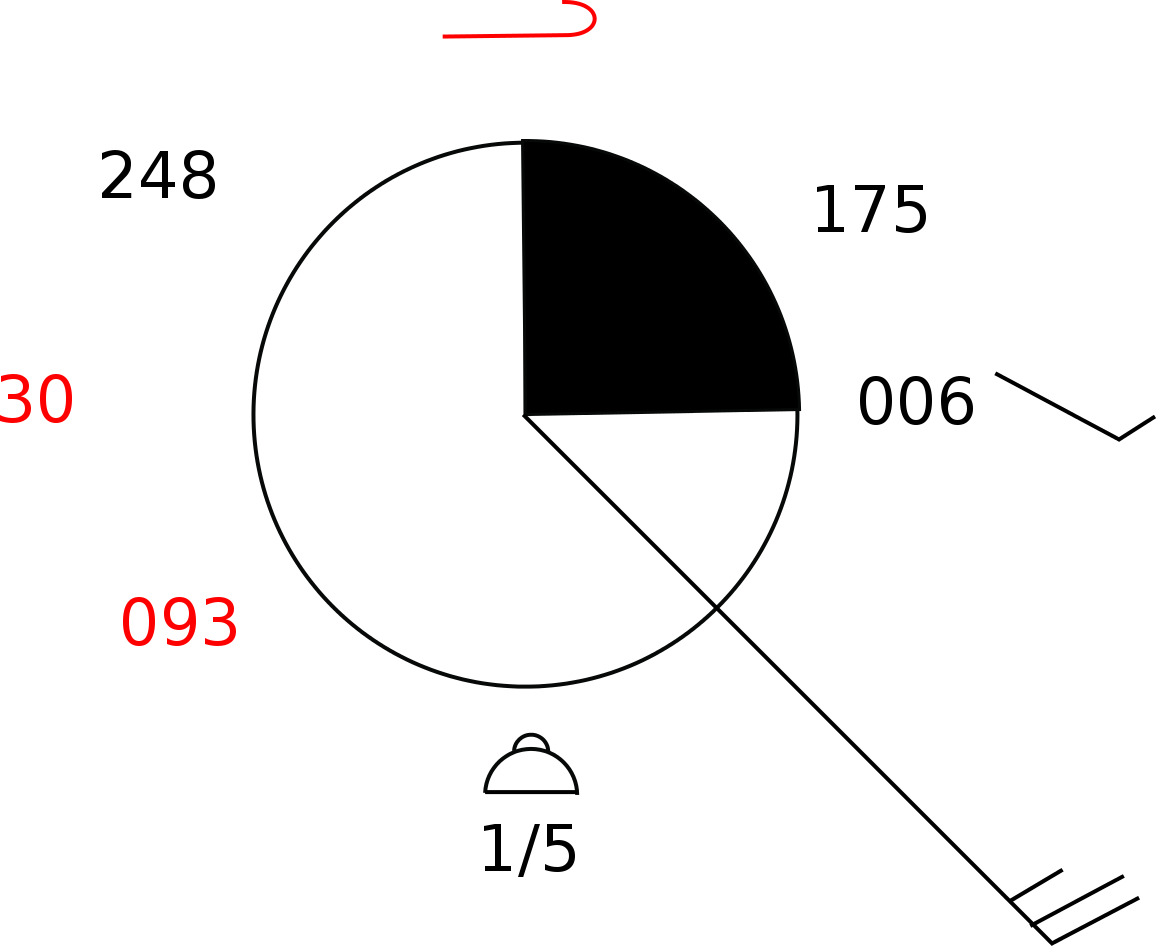
\includegraphics[width=0.3\textwidth]{Figs/drawing_synop.png}
\end{center}

%\newpage
\section{Exercises}
\paragraph{Exercise 1}
Given the sea level pressure field values draw the associated isobar lines. 

\paragraph{Exercise 2}
Given the surface pressure chart represented in the figure
fill the given table and find and label the following items:

\begin{center}
\begin{tabular}{ccc}
Cold front &	Col& Warm front\\
Trough     &Occlusion&	High pressure center\\
Low pressure trough&	Low pressure center& High pressure ridge\\
Warm sector & & \\
\end{tabular}
\end{center}

%\begin{table}[h]
\begin{center}{\large
\begin{tabular}{c|c|c|c|}
\hline
\hline
Location & Pressure in \si{mb} & Location & Pressure in \si{mb}\\
\hline
A & & E & \\ 
\hline
B &  & F & \\
\hline 
C & & G & \\
\hline 
D & & H & \\ 
\hline
\hline
\end{tabular}
}
\end{center}
%\caption{Exercise 2}\label{tab_ex2}
%\end{table}

\paragraph{Exercise 3}
Given the following SYNOP codes decipher them and encode them graphically.

\begin{tabular}{cccccccccccc}
%
%La Coruña & & & & & & & & & & \\
%
 08001  &  11430  &  82001  &  10108  & 20075 & &40310 & 51004 &
 69901  &  75022  &  8562X  &  \\
%
%<SYN Title='AAXX' TStamp='908539200' LatLon='36.783, 137.050' BId='47606'
%SName=', FUSHIK' SType='AUTO'>
%<SYID WS='4'>16124 47606</SYID>
%<SYG Vis='9000' Wind='200, 4' T='20.7' TD='19.7' P='998.5' P0='1000.0' Pd='3 4.2'
%Prec='7, 12' WX='8180' Tmx='27.4'>1//59 /2009 10207 20197 39985 40000 53042 60072 78180 333 10274</SYG>
%</SYN>
47606  &  11650 & 80516 & 10176 & 20141 & 39844 & 40104& 52020& 60092& 71022& 8552X \\
%
%
08180  & 32980&  43216  &  10154  &  21019  &  & 40154  &  50003 & & &
 83031 &    \\
%
%<SYN Title='AAXX' TStamp='908539200' LatLon='37.483, 130.900' BId='47115'
%SName=', ULLUNGDO ISLAND' Elev='223'>
%<SYID WS='4'>16124 47115</SYID>
%<SYG Ceiling='3000' Vis='5000' Wind='50, 8' T='17.6' TD='14.1' P='984.4' P0='1010.4' Pd='2 2.0'
%Prec='9, 12' WX='1022' Tmx='18.9' Clouds='8552/'>11650 80516 10176 20141 39844 40104 52020 60092 71022 8552/ 333 10189 31017 55000 70126 92064</SYG>
%</SYN>
%
03535 & 41470 & 82312 & 10077 & 20064 & & 40007 & 58012&  & 72165&  8682X  &  \\
%
08001 & 11430 & 82001 & 10108 & 20075 & & 40310 & 51004 & 69901  &
75022  &  8562X  &  \\
47662 & 12970 & 20203 & 10203 & 20151 & 30150 & 40193 &56005 &60001 &
& 80002 & \\
\end{tabular}


\begin{center}
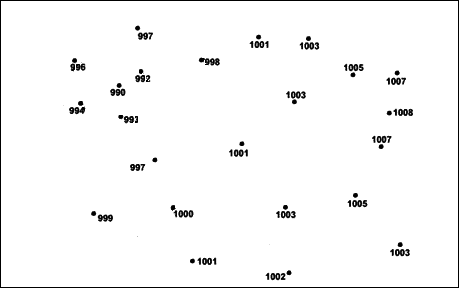
\includegraphics[angle=90,origin=c,width=0.8\textwidth]{Figs/parta_1.png}

\textbf{Exercise 1}. Sea level pressure values.
\end{center}

\begin{center}
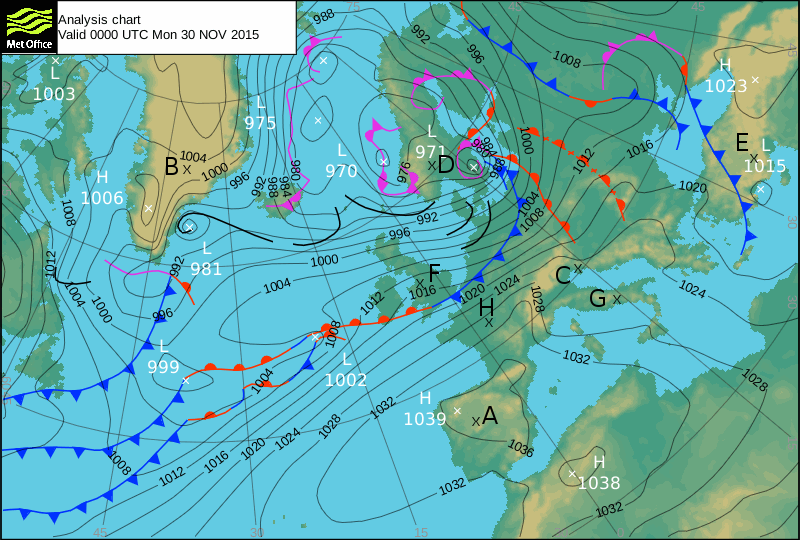
\includegraphics[angle=90,origin=c,width=0.8\textwidth]{Figs/map_ex_2.png}

\textbf{Exercise 2}. Met Office SYNOP Map.
\end{center}

%----------------------------------------------------------------------------------------

\nocite{rmetsoc}

%----------------------------------------------------------------------------------------

\bibliographystyle{abbrv}
%\bibliographystyle{apalike}

\bibliography{sample}

\appendix
\section{Appendix: SYNOP code graphical transcription}
\begin{figure}[h]
\begin{center}
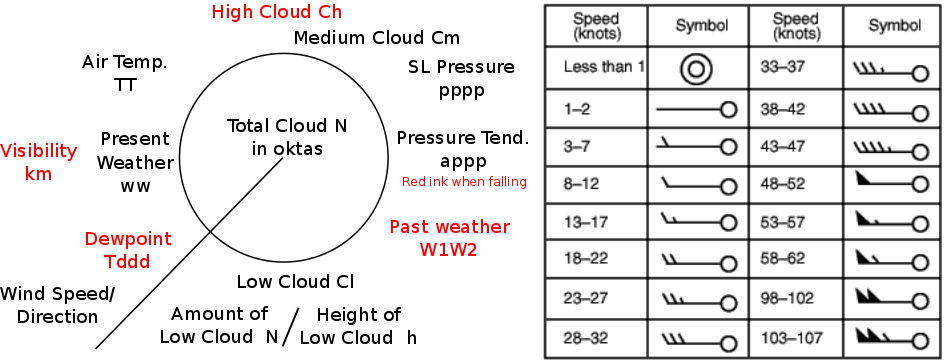
\includegraphics[width=0.9\textwidth]{Figs/circle_and_winds.png}
\caption{Left: Example of graphical codification of a SYNOP report. Black
  ink should be used unless otherwise stated. Right: Conventional codification for wind speed in a SYNOP report. Source: RMetS, The Royal Meteorological Society.}\label{circle_synop}
\end{center}
\end{figure}

\begin{figure}[h]
\begin{center}
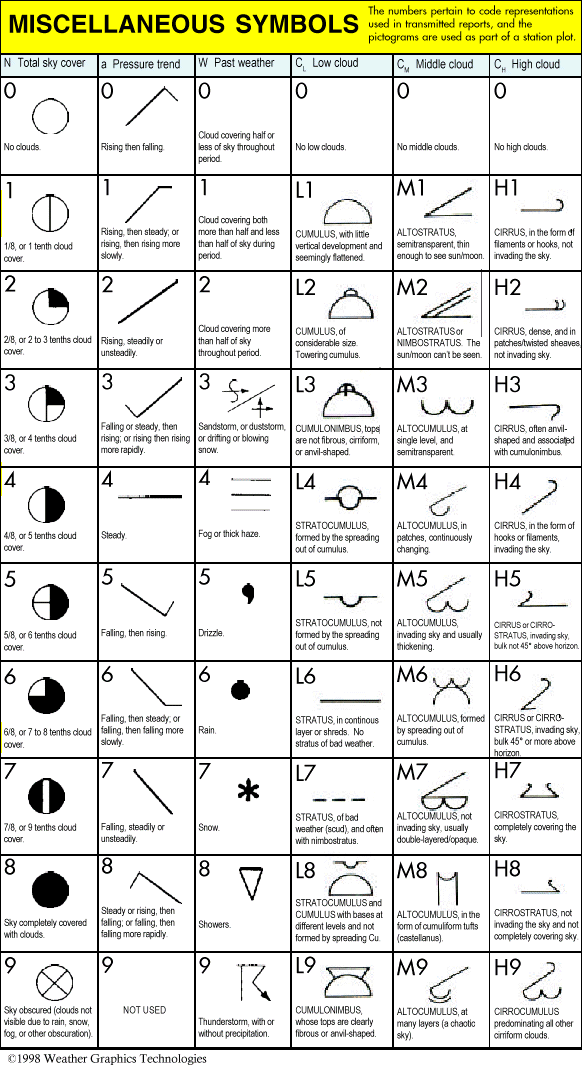
\includegraphics[width=0.7\textwidth]{Figs/wxcode2.png}
\caption{Example of standard graphical codification for cloud cover, pressure trend, past weather, and cloud types in a SYNOP report. Source: Weather Graphics Technologies.}\label{fig_synop_symbols_1}
\end{center}
\end{figure}

\begin{figure}[h]
\begin{center}
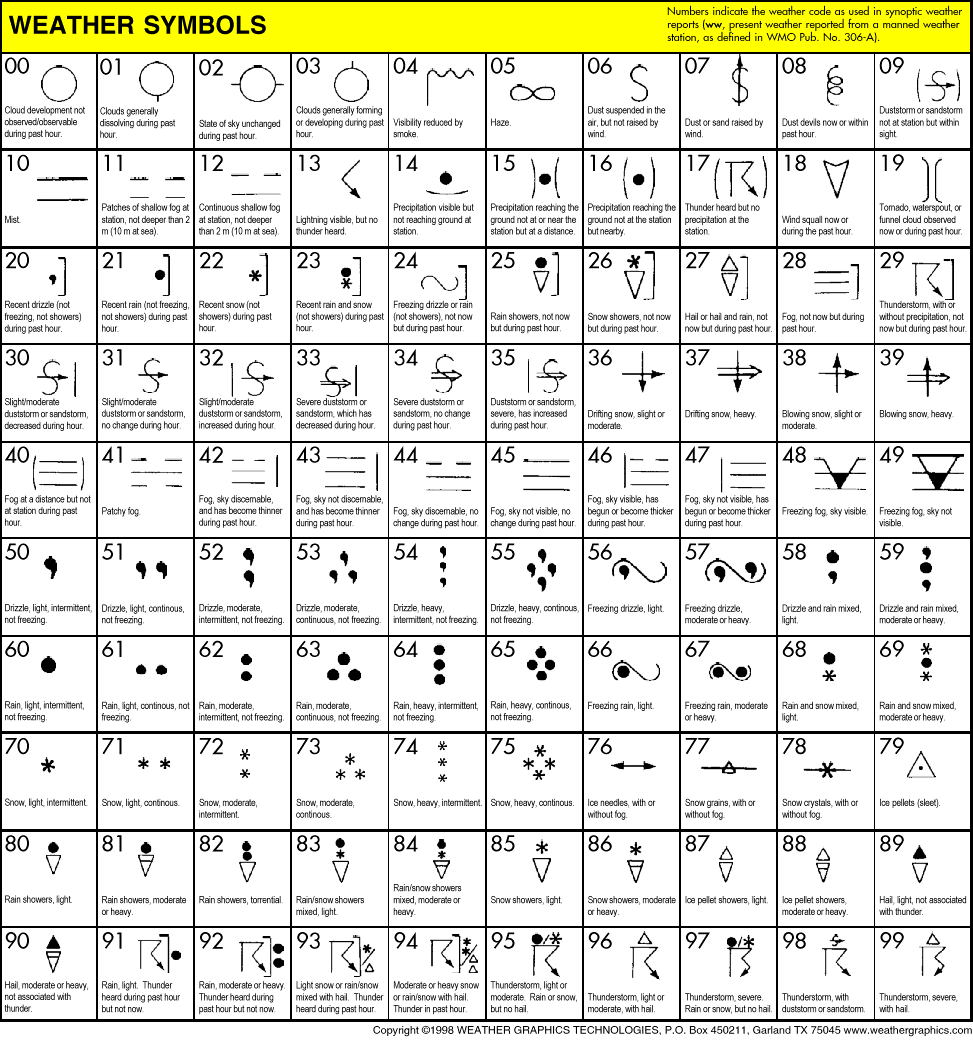
\includegraphics[width=0.95\textwidth]{Figs/wxcode1.png}
\caption{Example of standard graphical codification for present weather in a SYNOP report. Source: Weather Graphics Technologies.}\label{fig_synop_symbols_3}
\end{center}
\end{figure}

%----------------------------------------------------------------------------------------


\end{document}